\documentclass[runningheads,a4paper]{llncs}

\usepackage{amssymb}
\setcounter{tocdepth}{3}
\usepackage{graphicx}

\usepackage{url}
\newcommand{\keywords}[1]{\par\addvspace\baselineskip
  \noindent\keywordname\enspace\ignorespaces#1}

\begin{document}

\mainmatter  % start of an individual contribution

% first the title is needed
\title{ASGL}
\subtitle{Argumentation Semantics in Gecode and Lisp}

% a short form should be given in case it is too long for the running head
%\titlerunning{Score Manipulation in PWGL using KSQuant}

% the name(s) of the author(s) follow(s) next
%
% NB: Chinese authors should write their first names(s) in front of
% their surnames. This ensures that the names appear correctly in
% the running heads and the author index.
%
\author{Kilian Sprotte}

%
%\authorrunning{KSQuant - Complex Score Manipulation in PWGL through Quantization}
% (feature abused for this document to repeat the title also on left hand pages)

% the affiliations are given next; don't give your e-mail address
% unless you accept that it will be published
\institute{FernUniversit\"at in Hagen,\\
  Universit\"atsstra{\ss}e 47,\\
  58084 Hagen, Germany\\
  \email{kilian.sprotte@gmail.com}}

%
% NB: a more complex sample for affiliations and the mapping to the
% corresponding authors can be found in the file "llncs.dem"
% (search for the string "\mainmatter" where a contribution starts).
% "llncs.dem" accompanies the document class "llncs.cls".
%

%\toctitle{KSQuant - Complex Score Manipulation in PWGL through Quantization}
%\tocauthor{Score Manipulation in PWGL using KSQuant}
\maketitle

\newcommand{\asgl}{ASGL}

\newcommand{\grsem}{\textit{grounded semantics}}
\newcommand{\prsem}{\textit{preferred semantics}}
\newcommand{\stsem}{\textit{stable semantics}}
\newcommand{\cosem}{\textit{complete semantics}}

\begin{abstract}
  This paper presents the recent developments dealing with our
  metrical score representation format and how it can be used to
  produce and manipulate musical scores in PWGL. The base of these
  ideas is a special score format, called ENP-score-notation, that
  allows to describe in textual form various score elements like
  beats, measures, voices and parts. This basic format can be extended
  using keywords to represent other score attributes such as pitch,
  enharmonics, expressions, and so on, resulting in complete scores. A
  novel PWGL library, KSQuant, uses a similar format: instead of the
  tree-based representation of the metric structure, KSQuant uses a
  flat onset-time representation.  This format is ideal for many types
  of score manipulation operations where it is essential to preserve
  all score attributes.
\end{abstract}

\section{Introduction}\label{sec:introduction}

The plan of the paper is as follows. Section~\ref{sec:components}
presents libraries on which \asgl{} is built. Then, the realisation of
the computational tasks is exemplified w.r.t. \grsem{} in Section~
\ref{sec:grounded} and \prsem{} in Section~
\ref{sec:preferred}. Section~\ref{sec:reductions} details reductions
of queries performed by \asgl{} and Section~\ref{sec:conclusion} gives
a brief conclusion.

\section{System components}\label{sec:components}

\section{Grounded semantics}\label{sec:grounded}

\section{Preferred semantics}\label{sec:preferred}

\section{Reductions}\label{sec:reductions}

\section{Conclusion}\label{sec:conclusion}


\section{Sandbox}\label{sec:sandbox}
ASGL\cite{asgl} uses GECODE\cite{gecode} and ECL\cite{ecl}.


first-class computation spaces\cite{Engines:97}.


\section{Introduction}\label{old:sec:introduction}
Many different text-based formats have been developed for representing
the information in a musical score. Some typical examples are CMN,
GUIDO, MusiXTEX \cite{agon}, GNU LilyPond\cite{agon}, and
MusicXML \cite{agon}. Some Lisp-based representations are also
able to preserve only a subset of musical information, such as the
rhythm; these include the notation formats of both PatchWork \cite{agon}
and OpenMusic \cite{agon}. Our textual format, ENP-score-notation
\cite{agon}, also provides a way to generate and manipulate rich
musical data in PWGL \cite{agon}.  ENP-score-notation is offered as an
intermediate step between the score and the low-level file format. By
using ENP-score-notation, a score can be converted into a more
readable form that can also easily be converted back to an ENP
score. This kind of symmetry is beneficial, as it allows users to view
and modify score information without losing information.

The main topic of this paper is a novel PWGL user library, called
KSQuant~\cite{agon}, developed by Kilian Sprotte. KSQuant is
basically a quantizer, but unlike some of its predecessor libraries
found in PatchWork, OpenMusic and PWGL (e.g. OMKant and GRhythm), it
is strongly integrated in the PWGL system as it deals not only with
rhythmic structures, but also with other score attributes. Thus
KSQuant is closely related to ENP-score-notation. The main difference
between the systems is that whereas ENP-score-format deals normally
with metrical structures, KSQuant is duration/onset-time oriented.This
scheme allows KSQuant to be used as a high-level manipulation tool: it
can realize besides quantizing tasks also other complex patch-level
operations such as splitting and merging scores without loosing the
connection to other score parameters.

\section{KSQuant  Format}\label{old:KSQuant format}
KSQuant operates with a format called 'simple-format'. Instead of
using a tree-like structure like in ENP, events start at a certain
time point and their duration is specified by the time that passes
until the next event occurs. The ENP format is more expressive when it
comes to the exact description of rhythmical structures -- the
simple-format can be seen as a possible reduction.
\\
\\
To this purpose, KSQuant provides mainly two conversion functions:
\begin{itemize}
\item \texttt{score2simple} transforms a given ENP score into the
  simple-format.  In order to do this, no additional parameters are
  required.
\item \texttt{simple2score} is a much more complex function. It takes
  a lot of additional arguments to provide for information that is
  actually missing in the simple-format, such as
  time-signatures. Other parameters tune the quantization process that
  might need to be applied (Sect.~\ref{old:KSQuant Quantitizer}).
\end{itemize}

As an example, let us consider the score in Fig.~\ref{old:fig:enp-ex1}. It
is quite minimal, but demonstrates some important properties of the
ENP format. Concerning its rhythmical expressiveness, there is clearly
more information inherent in the specific notation of the two
triplets, than just a sequence of durations. Without changing them,
the second triplet could be re-notated as a sixtuplet, or as two
triplets with a tie in between.  It also shows the use of some
notational attributes. The accent is added to an entire chord, the
\texttt{x}-note-head attribute affects individual notes only.

\begin{figure}
  \centering
  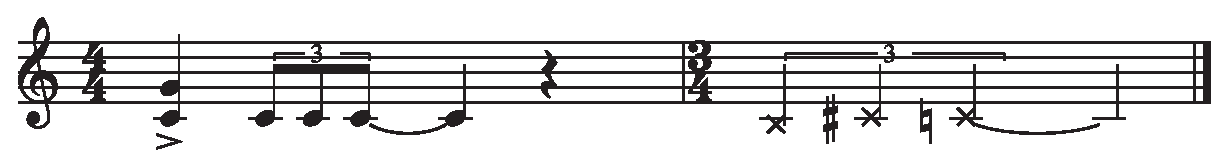
\includegraphics[width=9cm]{enp-ex1}
  \caption{A simple score using ENP that nevertheless demonstrates its
    ability to add notational attributes to a skeleton based on rhythm
    and pitch.}
  \label{old:fig:enp-ex1}
\end{figure}

The textual description in ENP-score-notation format of this score is
as follows:

\begin{scriptsize}
\begin{verbatim}
(((((1 ((1 :notes (67 60) :expressions (:accent))))
    (1 ((1 :notes (60)) (1 :notes (60)) (1 :notes (60))))
    (1 ((1.0 :notes (60))))
    (1 ((-1 :notes (60))))
    :time-signature (4 4))
   ((2
     ((1 :notes ((59 :note-head :x)))
      (1 :notes ((61 :note-head :x)))
      (1 :notes ((60 :note-head :x)))))
    (1 ((1.0 :notes ((60 :note-head :x)))))
    :time-signature
    (3 4)))))

\end{verbatim}
\end{scriptsize}

The tree-like structure used to represent the rhythmical groupings is
clearly visible. When this score is converted using
\texttt{score2simple}, the structure is translated to the following
flatter representation in simple-format:

\begin{scriptsize}
\begin{verbatim}
((((0.0 :notes (67 60) :expressions (:accent))
   (1.0 :notes (60))
   (1.333 :notes (60))
   (1.667 :notes (60))
   -3.0
   (4.0 :notes ((59 :note-head :x)))
   (4.667 :notes ((61 :note-head :x)))
   (5.333 :notes ((60 :note-head :x)))
   7.0)))
\end{verbatim}
\end{scriptsize}

The only rhythmical information that is left is the onset-time of each
event (chord\footnote{Technically, a single note object is always
  contained in a chord object.}  or rest), given as the first
floating-point number in each list. There is no notion of ties in the
simple-format\footnote{although this might be added to allow for the
  representation of partially tied chords}, so that tied chords in the
ENP-score-notation will be merged to a single event, which is broken
up again (possibly under different metrical circumstances) when
converting back. \\
Rests are represented explicitly by giving them a negative
onset-time. From this follows that durations are represented
implicitly; they are defined to be the inter-onset difference between
the onset-time of an event and the onset-time of its successor. For
the purpose of defining the last event's duration, an additional
time-value is added to the event-list specifying its
end-time and exceptionally not representing an event.

On the other hand, all attribute information is exactly preserved as
is. This allows the conversion processes to be reversible in the
attribute domain, while being subject to change in the rhythmical
domain in the case of \texttt{simple2score}.

\section{KSQuant  as a Quantizer}\label{old:KSQuant Quantitizer}
There has been a lot of ongoing research about Rhythm Quantization,
especially in the context of Automatic Music Transcription
\cite{agon}.  Starting from the naive model of grid
quantization, where each onset is quantized to the nearest grid point
independent of its neighbours, more elaborate models have been
developed that take the context into account. On the micro level the
goal is then to successfully recognize expressive deviations, whereas
tempo extraction on the macro level is performed.

KSQuant takes an intermediate position in this respect. Its
quantization algorithm is currently not as sophisticated as it could
be. The tempo, for instance, needs to be specified beforehand and can
not automatically be extracted from the input.  While there is
certainly a potential for future work, it should be emphasized that
the main goal of KSQuant is not to aid in Automatic Transcription, but
to provide means for score transformations that are much more easily
conducted on the simple-format representation than on the hierarchical
tree representation.

Nevertheless, the quantizer of KSQuant, as present in the function
\texttt{simple2score}, features a number of parameters, whose default
settings are shown in Fig.~\ref{old:fig:enp-ex1}.  Most important
is the set of permitted divisions, $PermDivs$ that is for convenience
controlled by the parameters $MaxDiv$ and $ForbiddenDivs$:
$$PermDivs = \{d:d \in \{1,2, ..., MaxDiv \}, d \notin ForbiddenDivs\}$$

Together with the tempo, $PermDivs$ establish a set of possible grids
that is evaluated for every group (the group length depending on the
time signature) by a simple heuristic employing the mean squared error
of onset deviation in that group.  The level of control provided by
$PermDivs$ often proves to be too limited. Therefore the user can
still finetune the result using the argument
$ForbiddenPatts$. Fig.~\ref{old:fig:enp-ex1} shows an example where the first
measure is quantized using only $MaxDiv$ = 8 (i.e. $ForbiddenPatts$ is
nil). The second measure is, however, quantized with $ForbiddenPatts$
set equal to \texttt{((1/16 3/32 3/32))} that forces the quantizer to
change the second beat.

%% \begin{figure}
%%   \centering
%%   \includegraphics[width=4cm]{simple2score-box}
%%   \caption{The \texttt{simple2score} box with completely opened additional inputs.}
%%   \label{fig:simple2score-box}
%% \end{figure}

%% \begin{figure}
%%   \centering
%%   \includegraphics[width=7cm]{fig3}
%%   \caption{The effect of using the $ForbiddenPatts$ argument.}
%%   \label{fig:fig3}
%% \end{figure}

\section{Score Manipulation}\label{old:Score Manipulation}
This section enumerates some examples that demonstrate how KSQuant
can be used to manipulate and build metrical scores. Often these
manipulations would be tedious to perform using the standard
ENP-score-notation format or other score building tools provided by
PWGL.

Fig.~\ref{old:fig:enp-ex1} gives a typical quantizing patch example where
onset-times and pitch information is given in simple-format to the
\texttt{simple2score} box. The result is fed in turn to a
\texttt{Score-Editor} box. Note that the simple-format allows to
specify the enharmonic spelling of the sixth note and that this
information is preserved in the \texttt{simple2score} transformation.

%% \begin{figure}
%%   \centering
%%   \includegraphics[width=10.5cm]{fig4}
%%   \caption{A patch example that unites pitch information with a
%%     quantizing operation.}
%%   \label{fig:fig4}
%% \end{figure}

In Fig.~\ref{old:fig:enp-ex1}, in turn, we have two input scores that are first merged to
a single voice (to the left), and then appended resulting in a two
measure score (to the right). We use here two KSQuant library boxes,
\texttt{simple-merge} and \texttt{simple-append}, that accept as
inputs the simple-format.

The append case in this example is trivial due to the fact that the
input items are entire bars. This operation could be easily performed
in other score editors, e.g. in Sibelius\cite{agon}. The more
complex case of joining multiple cells of varying duration is shown in
Fig.~\ref{old:fig:enp-ex1}. There is no need to mention that for a composer
this is quite a fundamental operation. Nevertheless -- in the context
of n-tuplets -- this has not been a well supported feature, e.g. by
Sibelius\footnote{Typically an error message would appear telling the
  user that it is not possible to insert a sequence in a metrical
  position where any n-tuplet of that sequence is divided by a
  bar line.}.

A similar problem arises, when we need to change the time-signatures
of a given passage. Again the presence of n-tuplets poses difficulties
when they need to be split across bar lines. Fig.~\ref{old:fig:enp-ex1}
demonstrates this case by changing the time-signature from
\texttt{4/4} to \texttt{3/8}. This leads to splitting the first
triplet and the second sixtuplet.

%% \begin{figure}
%%   \centering
%%   \includegraphics[width=12cm]{fig5}
%%   \caption{Simple merging and appending.}
%%   \label{fig:fig5}
%% \end{figure}

%% \begin{figure}
%%   \centering
%%   \includegraphics[width=12cm]{fig7}
%%   \caption{A more complex case of appending where the joints do not
%%     fall on the beat. Again, complex expressions are preserved.}
%%   \label{fig:fig7}
%% \end{figure}

%% \begin{figure}
%%   \centering
%%   \includegraphics[width=12cm]{fig8}
%%   \caption{Changing the time-signature to \texttt{3/8}. The n-tuplets
%%     are clearly affected by the new bar lines.}
%%   \label{fig:fig8}
%% \end{figure}

Our final example, shown in Fig.~\ref{old:fig:enp-ex1}, manipulates an input score by
scaling all offset-times by \texttt{5/8} (see the \texttt{scale} input of the
\texttt{simple2score} box). Note that also here the micro-tonal pitch
material is preserved.

%% \begin{figure}
%%   \centering
%%   \includegraphics[width=12cm]{fig6}
%%   \caption{An input score is scaled by \texttt{5/8} resulting in a new score.}
%%   \label{fig:fig6}
%% \end{figure}

\section{Future Work}
It has been shown that quantization allows to manipulate scores with
more ease compared to manipulating a hierarchical score structure.

The quantization algorithm of KSQuant potentially modifies the
onset-times of the input events (so that they can be notated with
given constraints). In the score manipulation examples of this paper,
however, no adjustment of onset-times and durations is required --
only a rearrangement of n-tuplets and ties is performed. Currently,
the user has no influence on how grouping decisons are being made;
this would be an interesting addition for the future.

Concerning the quantization part, it would be useful to report the
amount of modification to the user. A further step would allow to
specify a maximum deviation beforehand, thus allowing the user to
control the amount of quantization or even turn it off completely.

Additionally, it would be helpful to be able to specify multiple
parameter sets that would be active only in a certain region.

If this parametrization becomes even more detailed and
context-dependent, constraint-programming seems to become the
appropriate paradigm. Triplet divisions, for instance, could be
globally allowed, but not in immediate succession. With this
fine-grained control at hand, KSQuant would become an even better
suited tool for highly customized manipulations of rhythmical score
structures.

\section{Acknowledgement}
The work of Mikael Laurson and Mika Kuuskankare has been supported by
the Academy of Finland (SA 105557 and SA 114116).

\bibliography{bibdb}{}
\bibliographystyle{splncs03}

\end{document}
